\documentclass[12pt]{article}                                                                                                           
\usepackage[utf8]{inputenc}                                                                                                             
\usepackage[T1]{fontenc}                                                                                                                
\usepackage{amsmath, amssymb}                                                                                                           
\usepackage{geometry}                                                                                                                   
\usepackage{xcolor}                                                                                                                     
\usepackage{lipsum}                                                                                                                     
\usepackage{titlesec}                                                                                                                   
\usepackage{fancyhdr}                                                                                                                   
\usepackage{tcolorbox}                                                                                                                  
\usepackage{graphicx}                                                                                                                   
\usepackage{float}                                                                                      
\usepackage{tikz}
\usetikzlibrary{shapes.geometric, arrows.meta}
\usetikzlibrary{arrows.meta, decorations.markings}                                                                                      
                                                                                                                                        
\geometry{a4paper, margin=2.5cm}                                                                                                        
\pagestyle{fancy}                                                                                                                       
\fancyhf{}                                                                                                                              
\rhead{Problem Set I}                                                                                                                   
\lhead{Analysis V}                                                                                                                     
\cfoot{\thepage}                                                                                                                        
                                                                                                                                        
% Fancy titles                                                                                                                          
\titleformat{\section}{\normalfont\Large\bfseries}{Exercise \thesection:}{1em}{}                                                        
\titleformat{\subsection}{\normalfont\bfseries}{Correction:}{1em}{}                                                                     
                                                                                                                                        
% Custom box for correction
% If breakable doesn't work, we can simply remove it
\newtcolorbox{correctionbox}{                                                                                                           
  colback=gray!5,                                                                                                                       
  colframe=black,                                                                                                                       
  fonttitle=\bfseries,                                                                                                                  
  title=Correction,                                                                                                                     
  before skip=10pt,                                                                                                                     
  after skip=10pt                                                                                                                       
}                                                                                                                                       
                                                                                                                                        
% Fix headheight warning
\setlength{\headheight}{14.49998pt}

\begin{document}

% Cover info                                                                                                                            
\begin{center}
	\Large\textbf{Ibn Tofail University} \\[1em]
	\large\textit{Analysis V} \\[2em]
	\large\textit{Problem Set I} \\[0.5 em]
\end{center}

\vspace{1cm}

% ----------- EXERCISE 1 -------------                                                                                                  
\section{}
Show that:
$$|x+y| \le |x| + |y|, \quad \forall x, y \in \mathbb{R}^n$$


\begin{correctionbox}
    \begin{align*}
        \|a+b\|^2 &= \langle a+b,\,a+b \rangle \\
        &= \langle a,a \rangle + 2\langle a,b \rangle + \langle b,b \rangle \\ 
        &= \|a\|^2 + 2\langle a,b \rangle + \|b\|^2 \\
        &\leq \|a\|^2 + 2\|a\|\|b\| + \|b\|^2 \\
        &= (\|a\| + \|b\|)^2 \\
        \implies \|a+b\| &\leq \|a\| + \|b\| 
    \end{align*}
    \text{ive used C.S to prove it. (C.S : $|xy| \le |x||y|$)}
\end{correctionbox}

% ----------- EXERCISE 2 -------------                                                                                                  
\section{}
Let $||.||$ be the real function defined on $\mathbb{R}^{2}$ by:
$$||u=(x,y)|| = \sqrt{x^{2} + y^{2}}.$$
Show that this function satisfies:
$$||u+v|| \le ||u|| + ||v||, \quad \forall u, v \in \mathbb{R}^{2}$$


\begin{correctionbox}
    \text{This is just the same as exercise 1, but in $\mathbb{R}^2$}
\end{correctionbox}

\newpage

% ----------- EXERCISE 3 -------------                                                                                                  
\section{}
Let $X=(x_{1}, \ldots, x_{n}) \in \mathbb{R}^{n}$. We consider the following applications:
\begin{itemize}
    \item The $\mathbf{N_{1}}$-norm (or Manhattan norm):
    $$N_{1}(X) = \sum_{i=1}^{n} |x_{i}|$$
    \item The $\mathbf{N_{2}}$-norm (or Euclidean norm):
    $$N_{2}(X) = \sqrt{\sum_{i=1}^{n} |x_{i}|^{2}}$$
    \item The $\mathbf{N_{\infty}}$-norm (or maximum norm):
    $$N_{\infty}(X) = \sup_{i=1, \ldots, n} |x_{i}|$$
\end{itemize}
Show that the three preceding applications are norms on $\mathbb{R}^{n}$.


\begin{correctionbox}
    \begin{enumerate}
        \item The Three Norms verifies the first condition all of them are positive and when $X=0 \iff N(X) = 0$. (it's obvious)
        \item The Three Norms verifies the second condition all of them are absolutely scalable. (again it's obvious)
        \item The Three Norms verifies the third condition (Triangle inequality) all of them satisfy: $N(X+Y) \le N(X) + N(Y)$.  \end{enumerate}
    \text{For $N_1$ and $N_\infty$ it's obvious, for $N_2$ we can use C.S inequality to prove it.}
\end{correctionbox}

% ----------- EXERCISE 4 -------------                                                                                                   
\section{}
Show that the preceding norms satisfy the following properties:
\begin{enumerate}
    \item $N_{\infty}(X) \le N_{1}(X) \le n N_{\infty}(X)$
    \item $N_{\infty}(X) \le N_{2}(X) \le \sqrt{n} N_{\infty}(X)$
    \item $\frac{1}{n} N_{1}(X) \le N_{2}(X) \le \sqrt{n} N_{1}(X)$
\end{enumerate}


\begin{correctionbox}
\begin{enumerate}
    \item Since \( N_\infty(X) = |x_{i_0}| \) for some \( i_0 \),
    \[
    N_1(X) = \sum_{i=1}^n |x_i| \geq |x_{i_0}| = N_\infty(X),
    \]
    and since \( |x_i| \leq N_\infty(X) \) for all \( i \),
    \[
    N_1(X) = \sum_{i=1}^n |x_i| \leq \sum_{i=1}^n N_\infty(X) = n\, N_\infty(X).
    \]

    \item Similarly,
    \[
    N_2(X)^2 = \sum_{i=1}^n |x_i|^2 \geq |x_{i_0}|^2 = N_\infty(X)^2 \implies N_2(X) \geq N_\infty(X),
    \]
    and
    \[
    N_2(X)^2 = \sum_{i=1}^n |x_i|^2 \leq \sum_{i=1}^n N_\infty(X)^2 = n\, N_\infty(X)^2 \implies N_2(X) \leq \sqrt{n}\, N_\infty(X).
    \]

    \item By the Cauchy--Schwarz inequality,
    \[
    \left( \sum_{i=1}^n |x_i| \cdot 1 \right)^2 \leq \left( \sum_{i=1}^n |x_i|^2 \right) \left( \sum_{i=1}^n 1^2 \right) = n\, N_2(X)^2,
    \]
    so
    \[
    N_1(X)^2 \leq n\, N_2(X)^2 \implies N_2(X) \geq \frac{1}{\sqrt{n}} N_1(X) \geq \frac{1}{n} N_1(X).
    \]
    Also, since \( |x_i|^2 \leq |x_i| \cdot N_1(X) \) for each \( i \), 
    $N_2(X)^2 = \sum_{i=1}^n |x_i|^2 \leq N_1(X) \sum_{i=1}^n |x_i| = N_1(X)^2$ 
    $$\implies N_2(X) \leq N_1(X) \leq \sqrt{n}\, N_1(X)$$
\end{enumerate}
\end{correctionbox}

----------- EXERCISE 5 -------------                                                                                                   
% ----------- EXERCISE 5 -------------                                                                                                   
\section{}
In $\mathbb{R}^{2}$, draw the open balls of center $O$ and radius $1$, for each of the three usual norms.

\begin{correctionbox}
\begin{center}
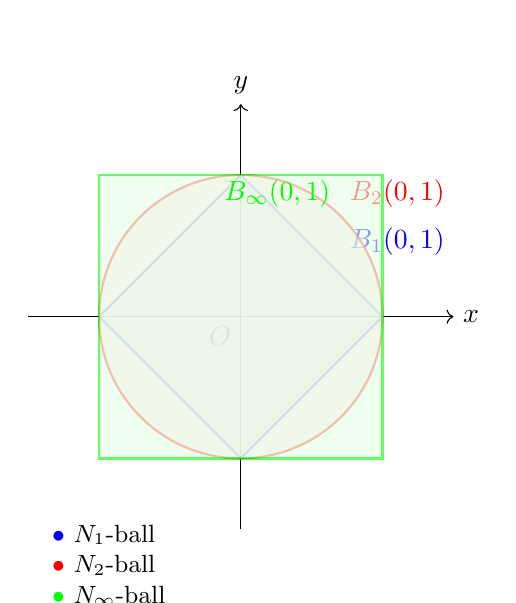
\begin{tikzpicture}[scale=1.8]
    \draw[->] (-1.5,0) -- (1.5,0) node[right] {$x$};
    \draw[->] (0,-1.5) -- (0,1.5) node[above] {$y$};
    \draw (0,0) circle (0pt) node[below left] {$O$};

    % N1 ball: diamond (L1 norm)
    \draw[thick, blue, fill=blue!10, opacity=0.6] 
        (-1,0) -- (0,1) -- (1,0) -- (0,-1) -- cycle;
    \node[blue, below right] at (0.7,0.7) {$B_1(0,1)$};

    % N2 ball: circle (Euclidean)
    \draw[thick, red, fill=red!10, opacity=0.6] (0,0) circle (1);
    \node[red, above right] at (0.7,0.7) {$B_2(0,1)$};

    % N∞ ball: square (max norm)
    \draw[thick, green, fill=green!10, opacity=0.6] 
        (-1,-1) rectangle (1,1);
    \node[green, above left] at (0.7,0.7) {$B_\infty(0,1)$};

% Legend
    \node[anchor=north west, text width=4cm, font=\small] at (-1.4,-1.4) {
        \textcolor{blue}{$\bullet$} $N_1$-ball \\
        \textcolor{red}{$\bullet$} $N_2$-ball \\
        \textcolor{green}{$\bullet$} $N_\infty$-ball
    };
\end{tikzpicture}
\end{center}

\bigskip

\noindent
\textbf{Explanation:}
\begin{enumerate}
    \item The $N_1$-ball is the set $ \{(x,y) : |x| + |y| < 1\} $.
    \item The $N_2$-ball is the set $ \{(x,y) : x^2 + y^2 < 1\} $.
    \item The $N_\infty$-ball is the set $ \{(x,y) : \max(|x|,|y|) < 1\} $.
\end{enumerate}
\end{correctionbox}




% ----------- EXERCISE 6 -------------                                                                                                   
\section{}
\begin{enumerate}
    \item Show that an open ball is an open set.
    \item Show that a closed ball is a closed set.
\end{enumerate}


\begin{correctionbox}
Let $(E, \|\cdot\|)$ be a normed vector space over $\mathbb{R}$ or $\mathbb{C}$. For any $a \in E$ and $r > 0$, define:

\begin{enumerate}
    \item Open ball: $ B(a,r) = \{ x \in E : \|x - a\| < r \} $
    \item Closed ball: $ \overline{B}(a,r) = \{ x \in E : \|x - a\| \leq r \} $
\end{enumerate}

\medskip

\textbf{1. An open ball is an open set.}

Let $ x_0 \in B(a,r) $. We must show there exists $ \varepsilon > 0 $ such that $ B(x_0, \varepsilon) \subseteq B(a,r) $.

Set $ \varepsilon = r - \|x_0 - a\| > 0 $ (since $ x_0 \in B(a,r) $).

Take any $ x \in B(x_0, \varepsilon) $. Then:
\[
\|x - a\| \leq \|x - x_0\| + \|x_0 - a\| < \varepsilon + \|x_0 - a\| = r.
\]
So $ x \in B(a,r) $, hence $ B(x_0, \varepsilon) \subseteq B(a,r) $.

Therefore, every point in $ B(a,r) $ has a neighborhood contained in it → $ B(a,r) $ is open.

\medskip

\textbf{2. A closed ball is a closed set.}

We show its complement is open. Let $ x_0 \notin \overline{B}(a,r) $, i.e., $ \|x_0 - a\| > r $.

Set $ \varepsilon = \|x_0 - a\| - r > 0 $.

Take any $ x \in B(x_0, \varepsilon) $. Then:
\[
\|x - a\| \geq \|x_0 - a\| - \|x - x_0\| > \|x_0 - a\| - \varepsilon = r.
\]
So $ x \notin \overline{B}(a,r) $, hence $ B(x_0, \varepsilon) \subseteq E \setminus \overline{B}(a,r) $.

Thus, the complement of $ \overline{B}(a,r) $ is open → $ \overline{B}(a,r) $ is closed.
\end{correctionbox}

% ----------- the documents finishes here body :D -------------                                                                         
\end{document}